\chapter{System design} \label{ch:sys_design}

	\hspace{15pt}First of all see the design in picture:

		\begin{figure}[h]
			\centering
			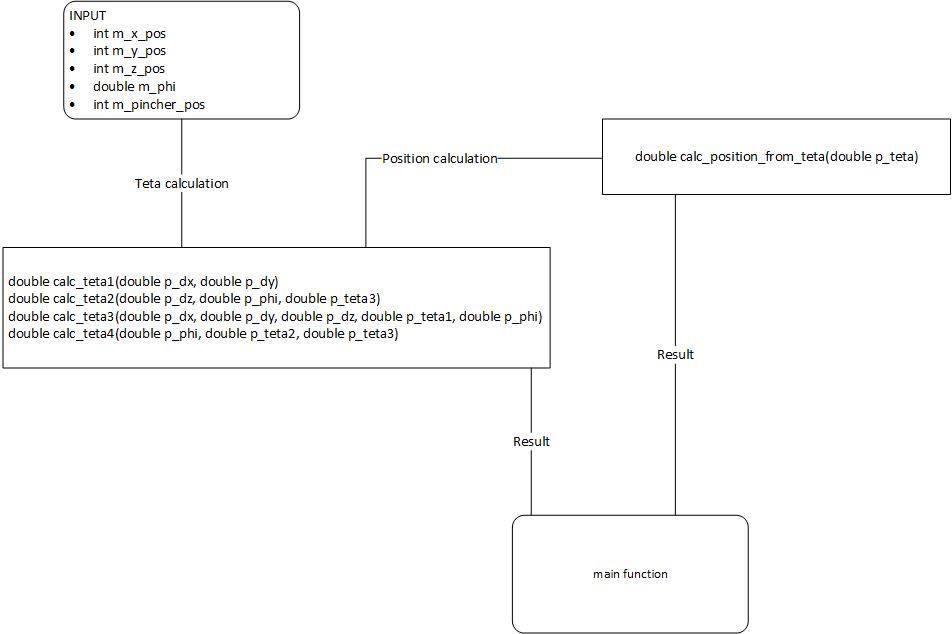
\includegraphics[width=\textwidth]{./images/system_design}
			\caption{System design}
		\end{figure}

	Generally about the Denavit-Hartenber parameters
For general description of robot geometry exist a method called Denavit-Hartenberger transformation matrix. With this a coordinate system can be transmitted in any coordinate system, if two offsets and two rotations are used in a corresponding order. In this case the two distance marked with d and a, and the rotation parameters are the following: $\theta$, q. \\



General steps:
	\begin{enumerate}
			\item Define the coordinate system for the wrists of the robot.\\
			\begin{enumerate}
				\item For the i and i+1 wrists take a rectangular coordinate system, so the origin of the coordinate system fits into the wrist centers. The z axes of the coordinate system points to the direction of wrists. \\
			\end{enumerate}
			\item Define the conventional parameters \\
			
			\begin{enumerate}
				\item First parameter: $q_i$ in case of rotation wrist this is the size of the angle between $x_i$ and $x_(i-1)$ axes. \\
				\item Second parameter: $d_i$:the distance of the normal transverse of the wrists. \\
				\item Third parameter: $a_i$: length of the distance of the i-th and (i+1)-th wrist axes. \\
				\item Fourth parameter:  $\alpha _i$: angle between $z_(i-1)$ axis of i-th wirst and $z_i$ axis of (i+1)-th  wirst. \\
			\end{enumerate}
		\end{enumerate}
		
		\begin{figure}[H]
			\centering
			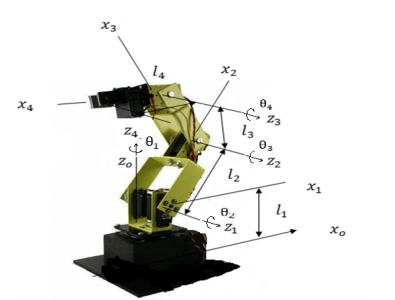
\includegraphics[]{./images/denavit_parameters}
			\caption{a. Denavit-Harzenbergeer parameters of the robot}
		\end{figure}
		
		\begin{enumerate}
			\item [3] The steps of matrix transformation: \\
		\end{enumerate} 

		\begin{figure}[H]
			\centering
			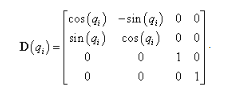
\includegraphics[]{./images/denavit1}
			\caption{a. Matrix transformation}
		\end{figure}
		\begin{figure}[H]
			\centering
			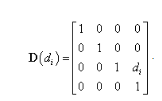
\includegraphics[]{./images/denavit2}
			\caption{b. Matrix transformation}
		\end{figure}
		\begin{figure}[H]
			\centering
			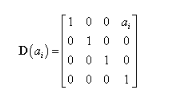
\includegraphics[]{./images/denavit3}
			\caption{c. Matrix transformation}
		\end{figure}
		\begin{figure}[H]
			\centering
			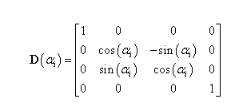
\includegraphics[]{./images/denavit4}
			\caption{d. Matrix transformation}
		\end{figure}
		\begin{figure}[H]
			\centering
			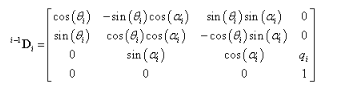
\includegraphics[]{./images/denavit5}
			\caption{e. Matrix transformation}
		\end{figure}
		
			
		The Denavit-Hartenberg parameters can be listed in a table as the follows:
		
			\begin{table}[h]
				\centering
				\begin{tabular}{|l|l|l|l|l|}
				\hline
				Frame (i) & $a_i$ & $\alpha _i$ & $d_i$ & $\theta _i$ \\ \hline
				1				&   0   &  90 & $I_1$ & $\theta _1$ \\ \hline
				2				&   $I_2$   &   0  & 0 & $\theta _2$ \\ \hline
				3				&   $I_3$   &   0  & 0 & $\theta _3$ \\ \hline
				4				&   $I_4$   &   0  & 0 & $\theta _4$ \\ \hline
				\end{tabular}
				\caption{Table of Denavit-Hartenberg parameters}
			\end{table}
			
			Our robots parameters is the following:
		
			\begin{table}[h]
				\centering
				\begin{tabular}{|l|l|}
				\hline
				Parameters & Robot parameters in mm \\ \hline
				$I_1$					 &       8                 \\ \hline
				$I_2$					 &       101                 \\ \hline
				$I_3$					 &       101                 \\ \hline
				$I_3$					 &       101                 \\ \hline
				\end{tabular}
				\caption{Table of robot parameters}
			\end{table}	
			
		In the end T matrix will specify the position and orientation of the robot in the standing coordinate system.
		After we have to using for this trigonometric formulas:
	
		\hspace{15pt}\[ dx = \cos\theta _1[l_2\times \cos \theta _2 + l_3\times \cos(\theta _2 + \theta _3)] + l_4\times \cos \theta _1 \times \cos(\theta _2 + \theta _3 + \theta _4) \]
		\hspace{15pt}\[ dy = \sin\theta _1[l_2\times \cos \theta _2 + l_3\times \cos(\theta _2 + \theta _3)] + l_4\times \sin \theta _1 \times \cos(\theta _2 + \theta _3 + \theta _4) \]
		\hspace{15pt}\[ dz = [l_1 + l_2\times \sin \theta _2 + l_3\times \sin(\theta _2 + \theta _3)] + l_4\times \sin(\theta _2 + \theta _3 + \theta _4) \]
		
		With the help of this parameters we can set the inverse kinematics on our robot as in the \ref{calculations}.
		
		